\documentclass[twoside]{book}

% Packages required by doxygen
\usepackage{fixltx2e}
\usepackage{calc}
\usepackage{doxygen}
\usepackage[export]{adjustbox} % also loads graphicx
\usepackage{graphicx}
\usepackage[utf8]{inputenc}
\usepackage{makeidx}
\usepackage{multicol}
\usepackage{multirow}
\PassOptionsToPackage{warn}{textcomp}
\usepackage{textcomp}
\usepackage[nointegrals]{wasysym}
\usepackage[table]{xcolor}

% Font selection
\usepackage[T1]{fontenc}
\usepackage[scaled=.90]{helvet}
\usepackage{courier}
\usepackage{amssymb}
\usepackage{sectsty}
\renewcommand{\familydefault}{\sfdefault}
\allsectionsfont{%
  \fontseries{bc}\selectfont%
  \color{darkgray}%
}
\renewcommand{\DoxyLabelFont}{%
  \fontseries{bc}\selectfont%
  \color{darkgray}%
}
\newcommand{\+}{\discretionary{\mbox{\scriptsize$\hookleftarrow$}}{}{}}

% Page & text layout
\usepackage{geometry}
\geometry{%
  a4paper,%
  top=2.5cm,%
  bottom=2.5cm,%
  left=2.5cm,%
  right=2.5cm%
}
\tolerance=750
\hfuzz=15pt
\hbadness=750
\setlength{\emergencystretch}{15pt}
\setlength{\parindent}{0cm}
\setlength{\parskip}{0.2cm}
\makeatletter
\renewcommand{\paragraph}{%
  \@startsection{paragraph}{4}{0ex}{-1.0ex}{1.0ex}{%
    \normalfont\normalsize\bfseries\SS@parafont%
  }%
}
\renewcommand{\subparagraph}{%
  \@startsection{subparagraph}{5}{0ex}{-1.0ex}{1.0ex}{%
    \normalfont\normalsize\bfseries\SS@subparafont%
  }%
}
\makeatother

% Headers & footers
\usepackage{fancyhdr}
\pagestyle{fancyplain}
\fancyhead[LE]{\fancyplain{}{\bfseries\thepage}}
\fancyhead[CE]{\fancyplain{}{}}
\fancyhead[RE]{\fancyplain{}{\bfseries\leftmark}}
\fancyhead[LO]{\fancyplain{}{\bfseries\rightmark}}
\fancyhead[CO]{\fancyplain{}{}}
\fancyhead[RO]{\fancyplain{}{\bfseries\thepage}}
\fancyfoot[LE]{\fancyplain{}{}}
\fancyfoot[CE]{\fancyplain{}{}}
\fancyfoot[RE]{\fancyplain{}{\bfseries\scriptsize Generated on Sun Dec 6 2015 17\+:16\+:40 for Projeto Paradigmas by Doxygen }}
\fancyfoot[LO]{\fancyplain{}{\bfseries\scriptsize Generated on Sun Dec 6 2015 17\+:16\+:40 for Projeto Paradigmas by Doxygen }}
\fancyfoot[CO]{\fancyplain{}{}}
\fancyfoot[RO]{\fancyplain{}{}}
\renewcommand{\footrulewidth}{0.4pt}
\renewcommand{\chaptermark}[1]{%
  \markboth{#1}{}%
}
\renewcommand{\sectionmark}[1]{%
  \markright{\thesection\ #1}%
}

% Indices & bibliography
\usepackage{natbib}
\usepackage[titles]{tocloft}
\setcounter{tocdepth}{3}
\setcounter{secnumdepth}{5}
\makeindex

% Custom commands
\newcommand{\clearemptydoublepage}{%
  \newpage{\pagestyle{empty}\cleardoublepage}%
}


%===== C O N T E N T S =====

\begin{document}

% Titlepage & ToC
\pagenumbering{roman}
\begin{titlepage}
\vspace*{7cm}
\begin{center}%
{\Large Projeto Paradigmas \\[1ex]\large 1.\+0 }\\
\vspace*{1cm}
{\large Generated by Doxygen 1.8.10}\\
\vspace*{0.5cm}
{\small Sun Dec 6 2015 17:16:40}\\
\end{center}
\end{titlepage}
\clearemptydoublepage
\tableofcontents
\clearemptydoublepage
\pagenumbering{arabic}

%--- Begin generated contents ---
\chapter{Pagina principal}
\label{index}Este é um projeto com o objetivo da aprendizagem em prática da utilização do Qt Creator para programação visual. Foi idealizado a construção de um jogo simples 2\+D para acerto ao alvo de modo a incentivar o estudo e prática da fisica classica, mais precisamente do movimento parabólico. O usuario tem com objetivo informar a velocidade inicial e o angulo, no qual supostamente deverá acertar o alvo e ver a simulação acontecer para checar se sua resposta estava certa. 
\chapter{Projeto\+Paradigmas}
\label{md__r_e_a_d_m_e}
Autor\+: Willian Kossmann da Silva

Este é um mini projeto de programação visual utilizado como avaliação de conhecimento da Disciplina de Paradgimas de Programação da Universidade Federal do Rio Grande do Norte.

O projeto idealizado foi a construção de um jogo simples de tiro ao alvo (estilo Angry\+Birds), porém que estimula a prática de calculos físicos utilizando variaveis do movimento parabolico para acertar o alvo. 
\chapter{Hierarchical Index}
\section{Class Hierarchy}
This inheritance list is sorted roughly, but not completely, alphabetically\+:\begin{DoxyCompactList}
\item Q\+Main\+Window\begin{DoxyCompactList}
\item \contentsline{section}{Main\+Window}{\pageref{class_main_window}}{}
\end{DoxyCompactList}
\item Q\+Widget\begin{DoxyCompactList}
\item \contentsline{section}{Desenha}{\pageref{class_desenha}}{}
\end{DoxyCompactList}
\end{DoxyCompactList}

\chapter{Class Index}
\section{Class List}
Here are the classes, structs, unions and interfaces with brief descriptions\+:\begin{DoxyCompactList}
\item\contentsline{section}{{\bf Desenha} \\*Classe para desenho dos objetos }{\pageref{class_desenha}}{}
\item\contentsline{section}{{\bf Main\+Window} \\*Classe para construção da tela principal }{\pageref{class_main_window}}{}
\end{DoxyCompactList}

\chapter{Class Documentation}
\section{Desenha Class Reference}
\label{class_desenha}\index{Desenha@{Desenha}}


Classe para desenho dos objetos.  




{\ttfamily \#include $<$desenha.\+h$>$}

Inheritance diagram for Desenha\+:\begin{figure}[H]
\begin{center}
\leavevmode
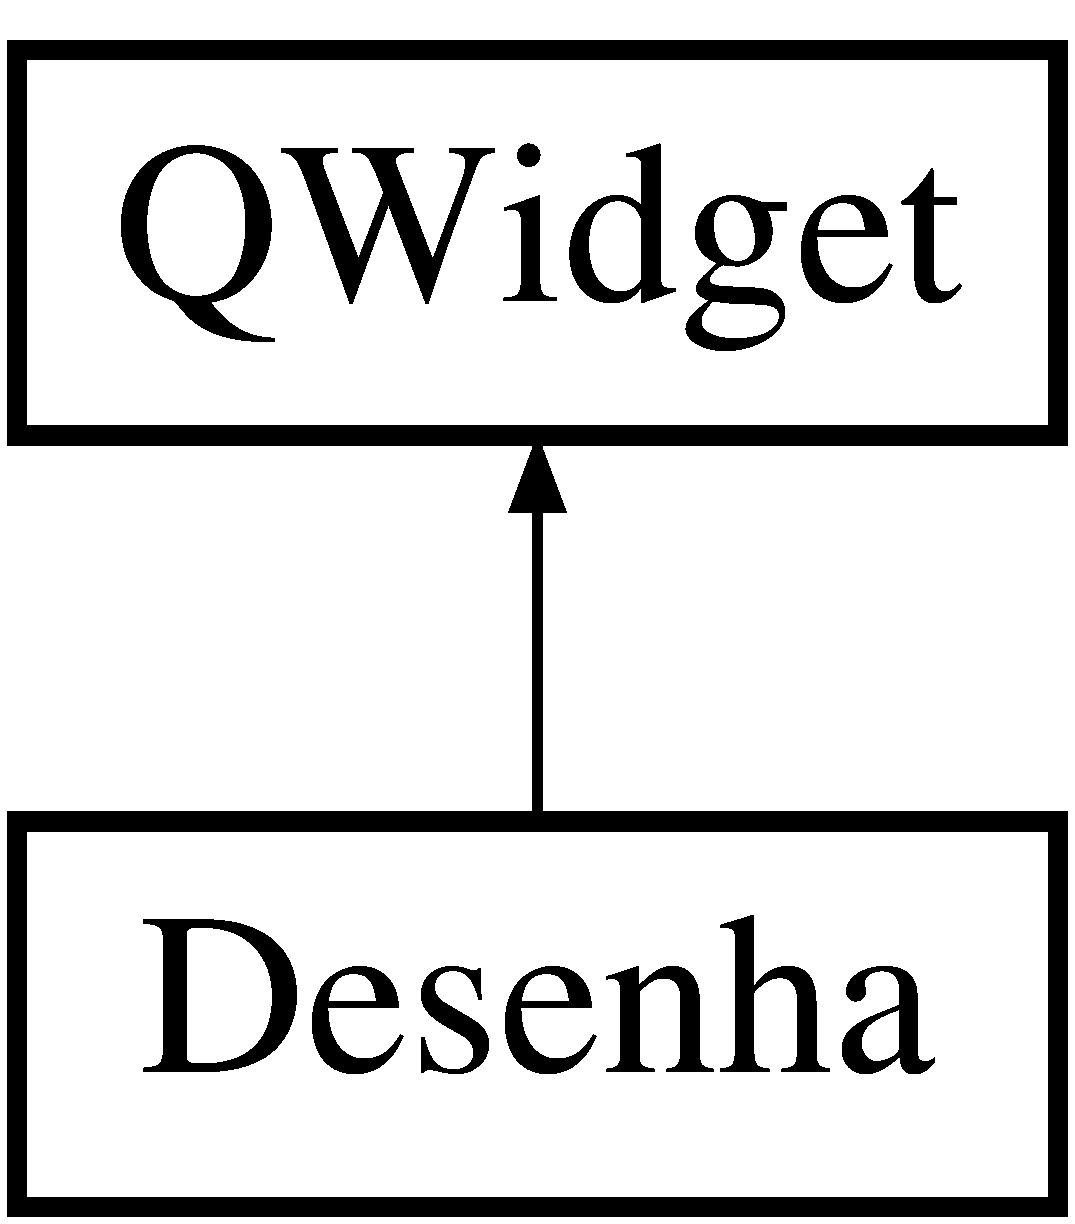
\includegraphics[height=2.000000cm]{class_desenha}
\end{center}
\end{figure}
\subsection*{Public Slots}
\begin{DoxyCompactItemize}
\item 
void {\bf muda\+\_\+velocidade} (Q\+String x)
\item 
void {\bf muda\+\_\+angulo} (Q\+String x)
\item 
void {\bf lancar} ()
\item 
void {\bf iniciar\+Jogo} ()
\end{DoxyCompactItemize}
\subsection*{Signals}
\begin{DoxyCompactItemize}
\item 
void {\bf display\+\_\+posicao\+X} (double)
\item 
void {\bf display\+\_\+posicao\+Y} (double)
\item 
void {\bf display\+\_\+status} (Q\+String)
\item 
void {\bf desativar\+\_\+botao} ()
\item 
void {\bf ativar\+\_\+botao} ()
\item 
void {\bf display\+\_\+pontuacao} (int)
\item 
void {\bf display\+\_\+recorde} (int)
\item 
void {\bf display\+\_\+vidas} (int)
\end{DoxyCompactItemize}
\subsection*{Public Member Functions}
\begin{DoxyCompactItemize}
\item 
{\bf Desenha} (Q\+Widget $\ast$parent=0)
\item 
void {\bf timer\+Event} ()
\item 
void {\bf paint\+Event} ()
\end{DoxyCompactItemize}
\subsection*{Public Attributes}
\begin{DoxyCompactItemize}
\item 
bool {\bf animacao\+Ativa}
\item 
double {\bf t}
\item 
double {\bf bala\+X}
\item 
double {\bf bala\+Y}
\item 
double {\bf alvo\+X}
\item 
double {\bf alvo\+Y}
\item 
double {\bf velocidade\+X}
\item 
double {\bf velocidade\+Y}
\item 
double {\bf velocidade\+Change}
\item 
double {\bf angulo\+Change}
\item 
int {\bf vidas\+Restantes}
\item 
int {\bf pontuacao\+Atual}
\item 
int {\bf pontuacao\+Recorde}
\end{DoxyCompactItemize}


\subsection{Detailed Description}
Classe para desenho dos objetos. 

Esta classe é responsável pelo processo dos dados de entrada ( velocidade e angulo ), para desenhar e dar movimento aos objetos do jogo (tela de fundo, canhao, alvo e bala) de acordo com os botôes de ativação. 

\subsection{Constructor \& Destructor Documentation}
\index{Desenha@{Desenha}!Desenha@{Desenha}}
\index{Desenha@{Desenha}!Desenha@{Desenha}}
\subsubsection[{Desenha(\+Q\+Widget $\ast$parent=0)}]{\setlength{\rightskip}{0pt plus 5cm}Desenha\+::\+Desenha (
\begin{DoxyParamCaption}
\item[{Q\+Widget $\ast$}]{parent = {\ttfamily 0}}
\end{DoxyParamCaption}
)\hspace{0.3cm}{\ttfamily [explicit]}}\label{class_desenha_a767ff68dbd895c972d890ff802aca599}
Construtor do objeto, com algumas pré-\/configurações em sua estrutura 

\subsection{Member Function Documentation}
\index{Desenha@{Desenha}!ativar\+\_\+botao@{ativar\+\_\+botao}}
\index{ativar\+\_\+botao@{ativar\+\_\+botao}!Desenha@{Desenha}}
\subsubsection[{ativar\+\_\+botao}]{\setlength{\rightskip}{0pt plus 5cm}void Desenha\+::ativar\+\_\+botao (
\begin{DoxyParamCaption}
{}
\end{DoxyParamCaption}
)\hspace{0.3cm}{\ttfamily [signal]}}\label{class_desenha_a6455059dc7f5815697ca5dd18716596c}
Sinal para controle do aparecimento do botão de lançar \index{Desenha@{Desenha}!desativar\+\_\+botao@{desativar\+\_\+botao}}
\index{desativar\+\_\+botao@{desativar\+\_\+botao}!Desenha@{Desenha}}
\subsubsection[{desativar\+\_\+botao}]{\setlength{\rightskip}{0pt plus 5cm}void Desenha\+::desativar\+\_\+botao (
\begin{DoxyParamCaption}
{}
\end{DoxyParamCaption}
)\hspace{0.3cm}{\ttfamily [signal]}}\label{class_desenha_a693d942b4b6aef4e3c7aec6be58ab081}
Sinal para controle do desparecimento do botão de lançar \index{Desenha@{Desenha}!display\+\_\+pontuacao@{display\+\_\+pontuacao}}
\index{display\+\_\+pontuacao@{display\+\_\+pontuacao}!Desenha@{Desenha}}
\subsubsection[{display\+\_\+pontuacao}]{\setlength{\rightskip}{0pt plus 5cm}void Desenha\+::display\+\_\+pontuacao (
\begin{DoxyParamCaption}
\item[{int}]{}
\end{DoxyParamCaption}
)\hspace{0.3cm}{\ttfamily [signal]}}\label{class_desenha_a32db4ab3f035c7074adb7710c80ae195}
Sinal para mostrar a pontuação atual da jogada \index{Desenha@{Desenha}!display\+\_\+posicao\+X@{display\+\_\+posicao\+X}}
\index{display\+\_\+posicao\+X@{display\+\_\+posicao\+X}!Desenha@{Desenha}}
\subsubsection[{display\+\_\+posicao\+X}]{\setlength{\rightskip}{0pt plus 5cm}void Desenha\+::display\+\_\+posicao\+X (
\begin{DoxyParamCaption}
\item[{double}]{}
\end{DoxyParamCaption}
)\hspace{0.3cm}{\ttfamily [signal]}}\label{class_desenha_adb456a18c0d1600f42477542843efe53}
Sinal para mostrar a posição atual do alvo, em X \index{Desenha@{Desenha}!display\+\_\+posicao\+Y@{display\+\_\+posicao\+Y}}
\index{display\+\_\+posicao\+Y@{display\+\_\+posicao\+Y}!Desenha@{Desenha}}
\subsubsection[{display\+\_\+posicao\+Y}]{\setlength{\rightskip}{0pt plus 5cm}void Desenha\+::display\+\_\+posicao\+Y (
\begin{DoxyParamCaption}
\item[{double}]{}
\end{DoxyParamCaption}
)\hspace{0.3cm}{\ttfamily [signal]}}\label{class_desenha_aebf5907c4ced8f67512852642d0e6aad}
Sinal para mostrar a posição atual do alvo, em Y \index{Desenha@{Desenha}!display\+\_\+recorde@{display\+\_\+recorde}}
\index{display\+\_\+recorde@{display\+\_\+recorde}!Desenha@{Desenha}}
\subsubsection[{display\+\_\+recorde}]{\setlength{\rightskip}{0pt plus 5cm}void Desenha\+::display\+\_\+recorde (
\begin{DoxyParamCaption}
\item[{int}]{}
\end{DoxyParamCaption}
)\hspace{0.3cm}{\ttfamily [signal]}}\label{class_desenha_a4bfa64c63f7cf0b5cb60682c06799682}
Sinal para mostrar a pontuação recorde do jogo \index{Desenha@{Desenha}!display\+\_\+status@{display\+\_\+status}}
\index{display\+\_\+status@{display\+\_\+status}!Desenha@{Desenha}}
\subsubsection[{display\+\_\+status}]{\setlength{\rightskip}{0pt plus 5cm}void Desenha\+::display\+\_\+status (
\begin{DoxyParamCaption}
\item[{Q\+String}]{}
\end{DoxyParamCaption}
)\hspace{0.3cm}{\ttfamily [signal]}}\label{class_desenha_a803cf36a39c17ce501133ad960f60346}
Sinal para amostrar a situação atual do jogador \index{Desenha@{Desenha}!display\+\_\+vidas@{display\+\_\+vidas}}
\index{display\+\_\+vidas@{display\+\_\+vidas}!Desenha@{Desenha}}
\subsubsection[{display\+\_\+vidas}]{\setlength{\rightskip}{0pt plus 5cm}void Desenha\+::display\+\_\+vidas (
\begin{DoxyParamCaption}
\item[{int}]{}
\end{DoxyParamCaption}
)\hspace{0.3cm}{\ttfamily [signal]}}\label{class_desenha_ad098f44a6dd67d686b2d45eea217ca33}
sinal para mostrar a quantidade de vidas restantes que o jogador possui \index{Desenha@{Desenha}!iniciar\+Jogo@{iniciar\+Jogo}}
\index{iniciar\+Jogo@{iniciar\+Jogo}!Desenha@{Desenha}}
\subsubsection[{iniciar\+Jogo}]{\setlength{\rightskip}{0pt plus 5cm}void Desenha\+::iniciar\+Jogo (
\begin{DoxyParamCaption}
{}
\end{DoxyParamCaption}
)\hspace{0.3cm}{\ttfamily [slot]}}\label{class_desenha_a4ad50ede3ea2e541c84d7e1b6cd75aa9}
Recebe o click do botao de incio de jogo \index{Desenha@{Desenha}!lancar@{lancar}}
\index{lancar@{lancar}!Desenha@{Desenha}}
\subsubsection[{lancar}]{\setlength{\rightskip}{0pt plus 5cm}void Desenha\+::lancar (
\begin{DoxyParamCaption}
{}
\end{DoxyParamCaption}
)\hspace{0.3cm}{\ttfamily [slot]}}\label{class_desenha_a83d16e71e64786ab6c86672e2f707b41}
Recebe o click do botao de lançamento \index{Desenha@{Desenha}!muda\+\_\+angulo@{muda\+\_\+angulo}}
\index{muda\+\_\+angulo@{muda\+\_\+angulo}!Desenha@{Desenha}}
\subsubsection[{muda\+\_\+angulo}]{\setlength{\rightskip}{0pt plus 5cm}void Desenha\+::muda\+\_\+angulo (
\begin{DoxyParamCaption}
\item[{Q\+String}]{x}
\end{DoxyParamCaption}
)\hspace{0.3cm}{\ttfamily [slot]}}\label{class_desenha_aa6b9c3ea8093510eef4835710ac80e1a}
Recebe o texto (Q\+String x) do line\+Edit Angulo a medida que ele vai sendo editado \index{Desenha@{Desenha}!muda\+\_\+velocidade@{muda\+\_\+velocidade}}
\index{muda\+\_\+velocidade@{muda\+\_\+velocidade}!Desenha@{Desenha}}
\subsubsection[{muda\+\_\+velocidade}]{\setlength{\rightskip}{0pt plus 5cm}void Desenha\+::muda\+\_\+velocidade (
\begin{DoxyParamCaption}
\item[{Q\+String}]{x}
\end{DoxyParamCaption}
)\hspace{0.3cm}{\ttfamily [slot]}}\label{class_desenha_a75b588272e3e4298d9817d84f8972c47}
Recebe o texto (Q\+String x) do line\+Edit Velocidade a medida que ele vai sendo editado \index{Desenha@{Desenha}!paint\+Event@{paint\+Event}}
\index{paint\+Event@{paint\+Event}!Desenha@{Desenha}}
\subsubsection[{paint\+Event()}]{\setlength{\rightskip}{0pt plus 5cm}void Desenha\+::paint\+Event (
\begin{DoxyParamCaption}
{}
\end{DoxyParamCaption}
)}\label{class_desenha_ae8c3e59e9db55e7b844137aa58ebb34a}
Membro da classe que controla o desenho na tela \index{Desenha@{Desenha}!timer\+Event@{timer\+Event}}
\index{timer\+Event@{timer\+Event}!Desenha@{Desenha}}
\subsubsection[{timer\+Event()}]{\setlength{\rightskip}{0pt plus 5cm}void Desenha\+::timer\+Event (
\begin{DoxyParamCaption}
{}
\end{DoxyParamCaption}
)}\label{class_desenha_a5dd232d3db7d17f9514b20c582556cf3}
Membro da classe que controla o timer\+Event, disparado a cada 1ms 

\subsection{Member Data Documentation}
\index{Desenha@{Desenha}!alvo\+X@{alvo\+X}}
\index{alvo\+X@{alvo\+X}!Desenha@{Desenha}}
\subsubsection[{alvo\+X}]{\setlength{\rightskip}{0pt plus 5cm}double Desenha\+::alvo\+X}\label{class_desenha_a7babe94d73aa0decdd02ddb4df2f97a1}
Posição x a ser desenhado o Alvo \index{Desenha@{Desenha}!alvo\+Y@{alvo\+Y}}
\index{alvo\+Y@{alvo\+Y}!Desenha@{Desenha}}
\subsubsection[{alvo\+Y}]{\setlength{\rightskip}{0pt plus 5cm}double Desenha\+::alvo\+Y}\label{class_desenha_aabec73afce4c1bef5b029803b2855857}
Posição y a ser desenhado o Alvo \index{Desenha@{Desenha}!angulo\+Change@{angulo\+Change}}
\index{angulo\+Change@{angulo\+Change}!Desenha@{Desenha}}
\subsubsection[{angulo\+Change}]{\setlength{\rightskip}{0pt plus 5cm}double Desenha\+::angulo\+Change}\label{class_desenha_aa59119fcf8884d6cf5a1f787cbfe3059}
Variavel auxiliar que é atualizada de acordo com a mudança do Line\+Edit Angulo \index{Desenha@{Desenha}!animacao\+Ativa@{animacao\+Ativa}}
\index{animacao\+Ativa@{animacao\+Ativa}!Desenha@{Desenha}}
\subsubsection[{animacao\+Ativa}]{\setlength{\rightskip}{0pt plus 5cm}bool Desenha\+::animacao\+Ativa}\label{class_desenha_ae3bdc380a414bb24af3525682e4cf32b}
Define se há movimento da bala a ser feito \index{Desenha@{Desenha}!bala\+X@{bala\+X}}
\index{bala\+X@{bala\+X}!Desenha@{Desenha}}
\subsubsection[{bala\+X}]{\setlength{\rightskip}{0pt plus 5cm}double Desenha\+::bala\+X}\label{class_desenha_a54b0658f3588ccd45cea5a7b9cca3dfa}
Posição x a ser desenhada a Bala \index{Desenha@{Desenha}!bala\+Y@{bala\+Y}}
\index{bala\+Y@{bala\+Y}!Desenha@{Desenha}}
\subsubsection[{bala\+Y}]{\setlength{\rightskip}{0pt plus 5cm}double Desenha\+::bala\+Y}\label{class_desenha_a9fa1e6e73def0d551768dace813fc558}
Posição y a ser desenhada a Bala \index{Desenha@{Desenha}!pontuacao\+Atual@{pontuacao\+Atual}}
\index{pontuacao\+Atual@{pontuacao\+Atual}!Desenha@{Desenha}}
\subsubsection[{pontuacao\+Atual}]{\setlength{\rightskip}{0pt plus 5cm}int Desenha\+::pontuacao\+Atual}\label{class_desenha_a566893dd512577f701f3296b9fd028a5}
Variavel de controle da pontuação durante um partida \index{Desenha@{Desenha}!pontuacao\+Recorde@{pontuacao\+Recorde}}
\index{pontuacao\+Recorde@{pontuacao\+Recorde}!Desenha@{Desenha}}
\subsubsection[{pontuacao\+Recorde}]{\setlength{\rightskip}{0pt plus 5cm}int Desenha\+::pontuacao\+Recorde}\label{class_desenha_a1af9232144a2e45fbda9f070173de673}
Variavel de controle da pontuação recorde (gravada em um arquivo) \index{Desenha@{Desenha}!t@{t}}
\index{t@{t}!Desenha@{Desenha}}
\subsubsection[{t}]{\setlength{\rightskip}{0pt plus 5cm}double Desenha\+::t}\label{class_desenha_a27c8e712de40b78ce378b6b3b1b323e1}
(Tempo) Variável auxiliar para calculo da altura da bala em cada instante \index{Desenha@{Desenha}!velocidade\+Change@{velocidade\+Change}}
\index{velocidade\+Change@{velocidade\+Change}!Desenha@{Desenha}}
\subsubsection[{velocidade\+Change}]{\setlength{\rightskip}{0pt plus 5cm}double Desenha\+::velocidade\+Change}\label{class_desenha_aafbb86ab55a0744d5cc091d53f981060}
Variavel auxiliar que é atualizada de acordo com a mudança do Line\+Edit Velocidade \index{Desenha@{Desenha}!velocidade\+X@{velocidade\+X}}
\index{velocidade\+X@{velocidade\+X}!Desenha@{Desenha}}
\subsubsection[{velocidade\+X}]{\setlength{\rightskip}{0pt plus 5cm}double Desenha\+::velocidade\+X}\label{class_desenha_a7982445d86436b2bfb927eda2141fc96}
Velocidade em x para calculo da posição \index{Desenha@{Desenha}!velocidade\+Y@{velocidade\+Y}}
\index{velocidade\+Y@{velocidade\+Y}!Desenha@{Desenha}}
\subsubsection[{velocidade\+Y}]{\setlength{\rightskip}{0pt plus 5cm}double Desenha\+::velocidade\+Y}\label{class_desenha_aaa45723dda585e775cd59ebf5a1968ba}
Velocidade em y para calculo da posição \index{Desenha@{Desenha}!vidas\+Restantes@{vidas\+Restantes}}
\index{vidas\+Restantes@{vidas\+Restantes}!Desenha@{Desenha}}
\subsubsection[{vidas\+Restantes}]{\setlength{\rightskip}{0pt plus 5cm}int Desenha\+::vidas\+Restantes}\label{class_desenha_abdb75d750c6aa4b0c09a3b7758f2c660}
Variavel de controle de vidas restantes para game over 

The documentation for this class was generated from the following files\+:\begin{DoxyCompactItemize}
\item 
desenha.\+h\item 
desenha.\+cpp\end{DoxyCompactItemize}

\section{Main\+Window Class Reference}
\label{class_main_window}\index{Main\+Window@{Main\+Window}}


Classe para construção da tela principal.  




{\ttfamily \#include $<$mainwindow.\+h$>$}

Inheritance diagram for Main\+Window\+:\begin{figure}[H]
\begin{center}
\leavevmode
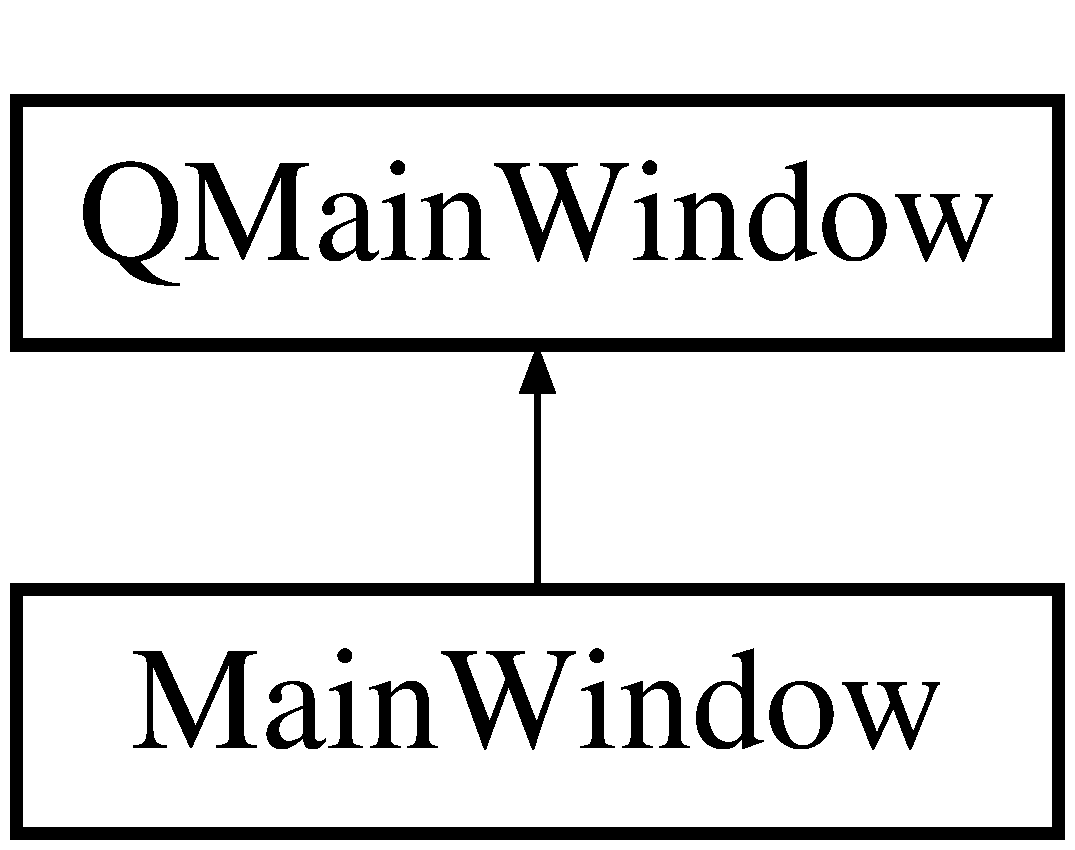
\includegraphics[height=2.000000cm]{class_main_window}
\end{center}
\end{figure}
\subsection*{Public Member Functions}
\begin{DoxyCompactItemize}
\item 
{\bf Main\+Window} (Q\+Widget $\ast$parent=0)
\item 
{\bf $\sim$\+Main\+Window} ()
\end{DoxyCompactItemize}


\subsection{Detailed Description}
Classe para construção da tela principal. 

Esta classe é responsável pela inicialização visual do programa e para construção dos demais objetos. 

\subsection{Constructor \& Destructor Documentation}
\index{Main\+Window@{Main\+Window}!Main\+Window@{Main\+Window}}
\index{Main\+Window@{Main\+Window}!Main\+Window@{Main\+Window}}
\subsubsection[{Main\+Window(\+Q\+Widget $\ast$parent=0)}]{\setlength{\rightskip}{0pt plus 5cm}Main\+Window\+::\+Main\+Window (
\begin{DoxyParamCaption}
\item[{Q\+Widget $\ast$}]{parent = {\ttfamily 0}}
\end{DoxyParamCaption}
)\hspace{0.3cm}{\ttfamily [explicit]}}\label{class_main_window_a8b244be8b7b7db1b08de2a2acb9409db}
Construtor da tela principal \index{Main\+Window@{Main\+Window}!````~Main\+Window@{$\sim$\+Main\+Window}}
\index{````~Main\+Window@{$\sim$\+Main\+Window}!Main\+Window@{Main\+Window}}
\subsubsection[{$\sim$\+Main\+Window()}]{\setlength{\rightskip}{0pt plus 5cm}Main\+Window\+::$\sim$\+Main\+Window (
\begin{DoxyParamCaption}
{}
\end{DoxyParamCaption}
)}\label{class_main_window_ae98d00a93bc118200eeef9f9bba1dba7}
Destrutor da tela principal 

The documentation for this class was generated from the following files\+:\begin{DoxyCompactItemize}
\item 
mainwindow.\+h\item 
mainwindow.\+cpp\end{DoxyCompactItemize}

%--- End generated contents ---

% Index
\backmatter
\newpage
\phantomsection
\clearemptydoublepage
\addcontentsline{toc}{chapter}{Index}
\printindex

\end{document}
